% !TEX root =  ../main.tex

%Probabilistic programming systems (PPS) allow probabilistic models to be represented in the form of a generative model and statements for conditioning on data \citep{carpenter2015stan,goodman_uai_2008,goodman_book_2014,mansinghka2014venture,minka_software_2010,wood2014new}.  
%%Informally, one can think of the generative model as the definition of a prior, the conditioning statements as the definition of a likelihood and the output of the program as samples from a posterior distribution. 
%Their core philosophy is to decouple model specification and inference, the former corresponding to the user-specified program code and the latter to an inference engine capable of operating on arbitrary programs.  Removing the need for users to write inference algorithms significantly reduces the burden of developing new models and makes effective statistical methods accessible to non-experts.
%%This inference engine must therefore be general purpose and robust, without making strong assumptions about the structure of the program, often taking the form of a Monte Carlo sampling scheme such as Markov chain Monte Carlo (MCMC) \citep{wingate2011lightweight}, Hamiltonian Monte Carlo \citep{carpenter2015stan}, sequential Monte Carlo (SMC) \citep{wood_aistats_2014} or particle MCMC \citep{van2015particle}.  
%
%Although significant progress has been made on the problem of general purpose \emph{inference} of program variables, less attention has been given to their \emph{optimization}.  Optimization is an essential tool for effective machine learning, necessary when the user requires a single estimate. It also often forms a tractable alternative when full inference is infeasible \citep{murphy2012machine}.  Moreover, coincident optimization and inference is often required, corresponding to a marginal maximum a posteriori (MMAP) setting where one wishes to maximize some variables, while marginalizing out others.  Examples of MMAP problems include hyperparameter optimization, expectation maximization, and policy search \citep{van2015black}.

%Here pure optimization, i.e. assuming the best possible possible environment, is clearly unsatisfactory, whilst inference alone is insufficient to determine the optimal action.

%Although significant progress has been made on the problem of general purpose \emph{inference} of program variables, less attention has been given to their \emph{optimization}. In many machine learning problems one might want to perform marginal maximum a posterior (MMAP) estimation to obtain a point estimate for a subset of random variables in a model while marginalizing over the remaining variables. Examples of such settings include hyperparameter optimization, decision making under uncertainty \cite{van2015black}, and problems where inference over top-level variables is either infeasible or the user simply desires a single point estimate \cite{murphy2012machine}.

%Even when these simulations are deterministic, this is an approximation to a truly probabilistic world. This setting corresponds to a MMAP framework, in which the user wishes to select the best design whilst marginalizing out the uncertainty about the environment or the simulation itself.

%To demonstrate how easily BOPP can be used, we present an application of optimal power allocation is shown in Figure \ref{fig:houses} with associated code in Figure \ref{fig:house-heating-code}.  Typically an engineer might try to solve this problem by making a number of fixed environmental assumptions and invoking a finite element simulation software, tuning by hand.  This process can be laborious and fails to capture the uncertainty in the environment.  BOPP provides a framework to naturally incorporate these uncertainties, whilst still exploiting the original simulation and returning a single solution the engineer can implement.

%In this paper we develop the first system that extends probabilistic program (PP) inference to a more general MMAP framework, wherein the user specifies a model in the same manner as existing systems, but then selects some subset of the sampled variables in the program to be optimized, with the rest marginalized using existing inference algorithms.  To do so, we define an \emph{optimization query}, which performs a program transformation to map unconditioned random variables onto conditioned random variables, whose values are passed to the transformed program as inputs. We then introduce Bayesian optimization for probabilistic programs (BOPP), a new framework for Gaussian process (GP) \citep{rasmussen2006gaussian} based  Bayesian optimization (BO) \citep{osborne2009gaussian, jones1998efficient} package integrated into the PPS Anglican \citep{wood2014new}. The BOPP method iteratively performs inference in a conditioned program using a generic method, such as sequential Monte Carlo (SMC), to obtain an unbiased estimate of the marginal likelihood of a conditioned program. Bayesian optimization of this marginal likelihood is then done by constructing a GP surrogate and maximizing the expected improvement \cite{brochu2010tutorial} to select values in a manner that balances exploration and exploitation. 
%
%In this paper we develop the first system that extends probabilistic programming (PP) to this more general MMAP framework, wherein the user specifies a model in the same manner as existing systems, but then selects some subset of the sampled variables in the program to be optimized, with the rest marginalized out using existing inference algorithms.  The \textit{optimization query} we introduce can be implemented and utilized in any PPS that supports an inference method returning a marginal likelihood estimate.  This framework increases the scope of models that can be expressed in PPS and gives additional flexibility in the outputs a user can request from the program.

%MMAP estimation is difficult as it corresponds to the optimization of an intractable integral, such that the optimization target is expensive to evaluate and gives noisy results.  Current PPS inference engines are typically unsuited to such settings.  We therefore introduce BOPP\footnote{Code available at {\small \url{http://www.github.com/probprog/bopp/}}}
%(Bayesian optimization for probabilistic programs) which couples existing inference algorithms from PPS, like \emph{Anglican} \citep{wood2014new}, with a new Gaussian process (GP) \citep{rasmussen2006gaussian} based Bayesian optimization (BO) package \citep{gutmann2016bayesian, jones1998efficient, osborne2009gaussian, shahriari2016unbounded}.  

To demonstrate the functionality provided by BOPP, we consider an example application of engineering design.  Engineering design relies extensively on simulations which typically have two things in common: the desire of the user to find a single best design and an uncertainty in the environment in which the designed component will live. Even when these simulations are deterministic, this is an approximation to a truly stochastic world. By expressing the utility of a particular design-environment combination using an approximate Bayesian computation (ABC) likelihood \citep{csillery2010approximate}, one can pose this as a MMAP problem, optimizing the design while marginalizing out the environmental uncertainty.\footnote{For the reasons explained in Section~\ref{sec:opt:intro},
	it will often be more
	convenient to use the risk minimization framework for engineering design because one generally wishes to place emphasis
	on rare catastrophic events.}
Figure~\ref{fig:houses} illustrates how BOPP can be applied to engineering design, taking the example of optimizing the distribution of power between radiators in a house so as to homogenize the temperature, while marginalizing out possible weather conditions and subject to a total energy budget. The Anglican program shown in Figure~\ref{fig:house-heating-code} allows us to define a prior over the uncertain weather, while conditioning on the output of a deterministic simulator (here Energy2D \citep{xie2012energy2d}-a finite element package for heat transfer) using an ABC likelihood.  BOPP now allows the required coincident inference and optimization to be carried out automatically, directly returning increasingly optimal configurations. 

\begin{figure*}[t]
	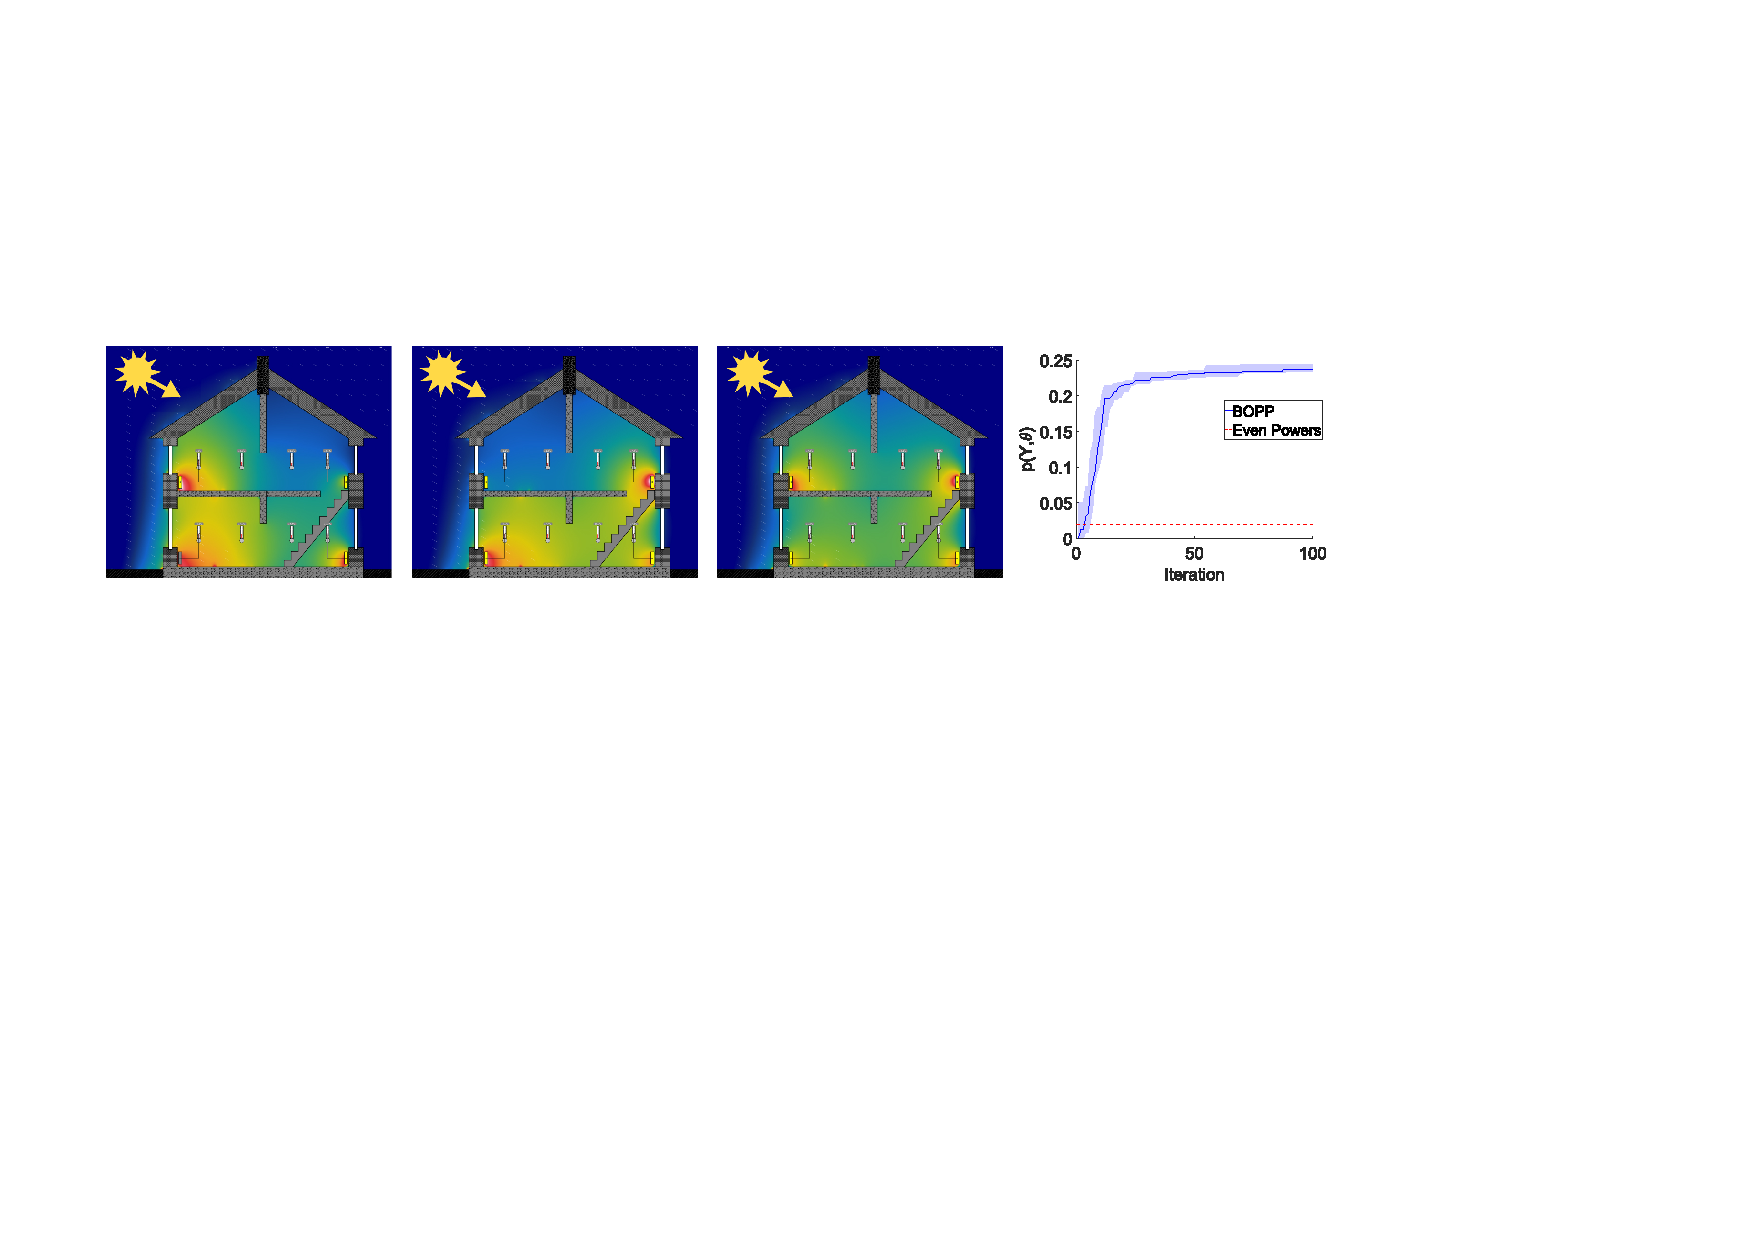
\includegraphics[width=\textwidth]{house-heating/combined_plot_rerun}
	\caption{
		\label{fig:houses}
		Simulation-based optimization of radiator powers subject to varying solar intensity. Shown are output heat maps from Energy2D \citep{xie2012energy2d} simulations at one intensity, corresponding from left to right to setting all the radiators to the same power, the best result from a set of randomly chosen powers, and the best setup found after 100 iterations of BOPP. The far right plot shows convergence of the evidence of the respective model, giving the median and 25/75\% quartiles.
	}
\end{figure*}

\begin{figure}[t]
	\vspace{5pt}
	\begin{lstlisting}[basicstyle=\ttfamily\small]
(defopt house-heating [alphas target-temps] [powers]
 (let [solar-intensity (sample weather-prior)
       powers (sample (dirichlet alphas))
       temps (simulate solar-intensity powers)]
  (observe (abc-likelihood temps) target-temps)))
	\end{lstlisting}	
	\vspace{-6pt}
	\caption{BOPP query for optimizing the power allocation to radiators in a house.  Here \lstinline{weather-prior} is a distribution over the solar intensity and a uniform Dirichlet prior with concentration \lsi{alpha} is placed over the powers. Calling \simulatec performs an Energy2D simulation of house temperatures. The utility of the resulting output is incorporated using \abcl, which measures a discrepency from the \texttt{target-temps}. Calling \doopt on this query invokes BOPP to perform MMAP estimation, with the second input \lstinline{powers} indicating the variable(s) to be optimized. Full details on the model and
		experiment are provided in~\cite{rainforth2017boppArxiv}.\label{fig:house-heating-code}}
	\vspace{-5pt}
\end{figure}

%Figure~\ref{fig:houses} illustrates how BOPP can be applied to engineering design, taking the example of optimizing the distribution of power between radiators in a house so as to homogenize the temperature, while marginalizing out possible weather conditions and subject to a total energy budget. The probabilistic program shown in Figure~\ref{fig:house-heating-code} allows us to define a prior over the uncertain weather, while conditioning on the output of a deterministic simulator (here Energy2D \citep{xie2012energy2d}-a finite element package for heat transfer) using an ABC likelihood.  BOPP now allows the required coincident inference and optimization to be carried out automatically, directly returning increasingly optimal configurations. 

BO is an attractive choice for the required optimization in MMAP as it is typically efficient in the number of target evaluations, operates on non-differentiable targets, and incorporates noise in the target function evaluations (see Section~\ref{sec:opt:BO}).  However, applying BO to probabilistic programs presents challenges, such as the need to give robust performance on a wide range of problems with varying scaling and potentially unbounded support.  Furthermore, the target program may contain unknown constraints, implicitly defined by the generative model, and variables whose type is unknown (i.e. they may be continuous or discrete).

On the other hand, the availability of the target source code in a PPS presents opportunities to overcome these issues and go beyond what can be done with existing BO packages.  BOPP exploits the source code in a number of ways, such as optimizing the acquisition function using the original generative model to ensure the solution satisfies the implicit constaints, performing adaptive domain scaling to ensure that GP kernel hyperparameters can be set according to problem-independent hyperpriors, and defining an adaptive non-stationary mean function to support unbounded BO. 

Together, these innovations mean that BOPP can be run in a manner that is fully black-box from the user's perspective, requiring only the identification of the target variables relative to current syntax for operating on arbitrary programs. We further show that BOPP is competitive with existing BO engines for direct optimization on common benchmarks problems that do not require marginalization.

%that can be implemented in any PPS where inference methods return marginal likelihood estimates. 



%MMAP estimation is generally difficult as it corresponds to the optimization of an intractable integral, such that function evaluations are expensive and give noisy results.  Current PPS inference engines are typically unsuited to such optimization.  We therefore introduce BOPP (Bayesian optimization for probabilistic programs) which couples existing inference algorithms with a new Gaussian process (GP) \citep{rasmussen2006gaussian} based Bayesian optimization (BO) \citep{osborne2009gaussian, jones1998efficient} package integrated into the PPS Anglican \citep{wood2014new}.  



%MMAP estimation for PPS presents further issues such as the need to be general purpose and robust, whilst dealing with potentially unknown constraints defined implicitly within the generative model.  


%On the other hand, the availability of the target source code in PPS presents opportunities to overcome these issues and go beyond what can be done with existing BO packages.  For example, it allows operation under unknown \emph{equality} constraints and applies automatic domain scaling for problem-independent GP hyperpriors.  In addition to delivering improved performance over prominent BO packages when used simply as an optimizer, these innovations mean that BOPP can be run in a manner that is fully black-box from the user's perspective, requiring only the identification of the target variables relative to current syntax for operating on arbitrary programs.

%\footnotetext{Though results are from the full BOPP implementation with sun heating marginalized out, the simulation plots correspond to a single common condition for the sun for visualization purposes.}

%\section{Motivating Example}
%\label{sec:motivation}


%The rest of this paper is outlined as follows: we first provide background on PPS, BO and GPs.  We define a framework for an optimization query and introduce our core code transformation to allow an arbitrary program to be optimized with respect to parameters defined within the program.  Our algorithm for optimizing the evidence of this program using BO and additional code transformations is outlined, we present experiments demonstrating the applicability of our method and we finish with concluding discussions and suggestions for future work.
